% prilohy

\chapter{Přílohy}

\cleartoleftpage
\section{Příloha A: Prvotní pravidla obsahující pouze proceduru hodnocení}
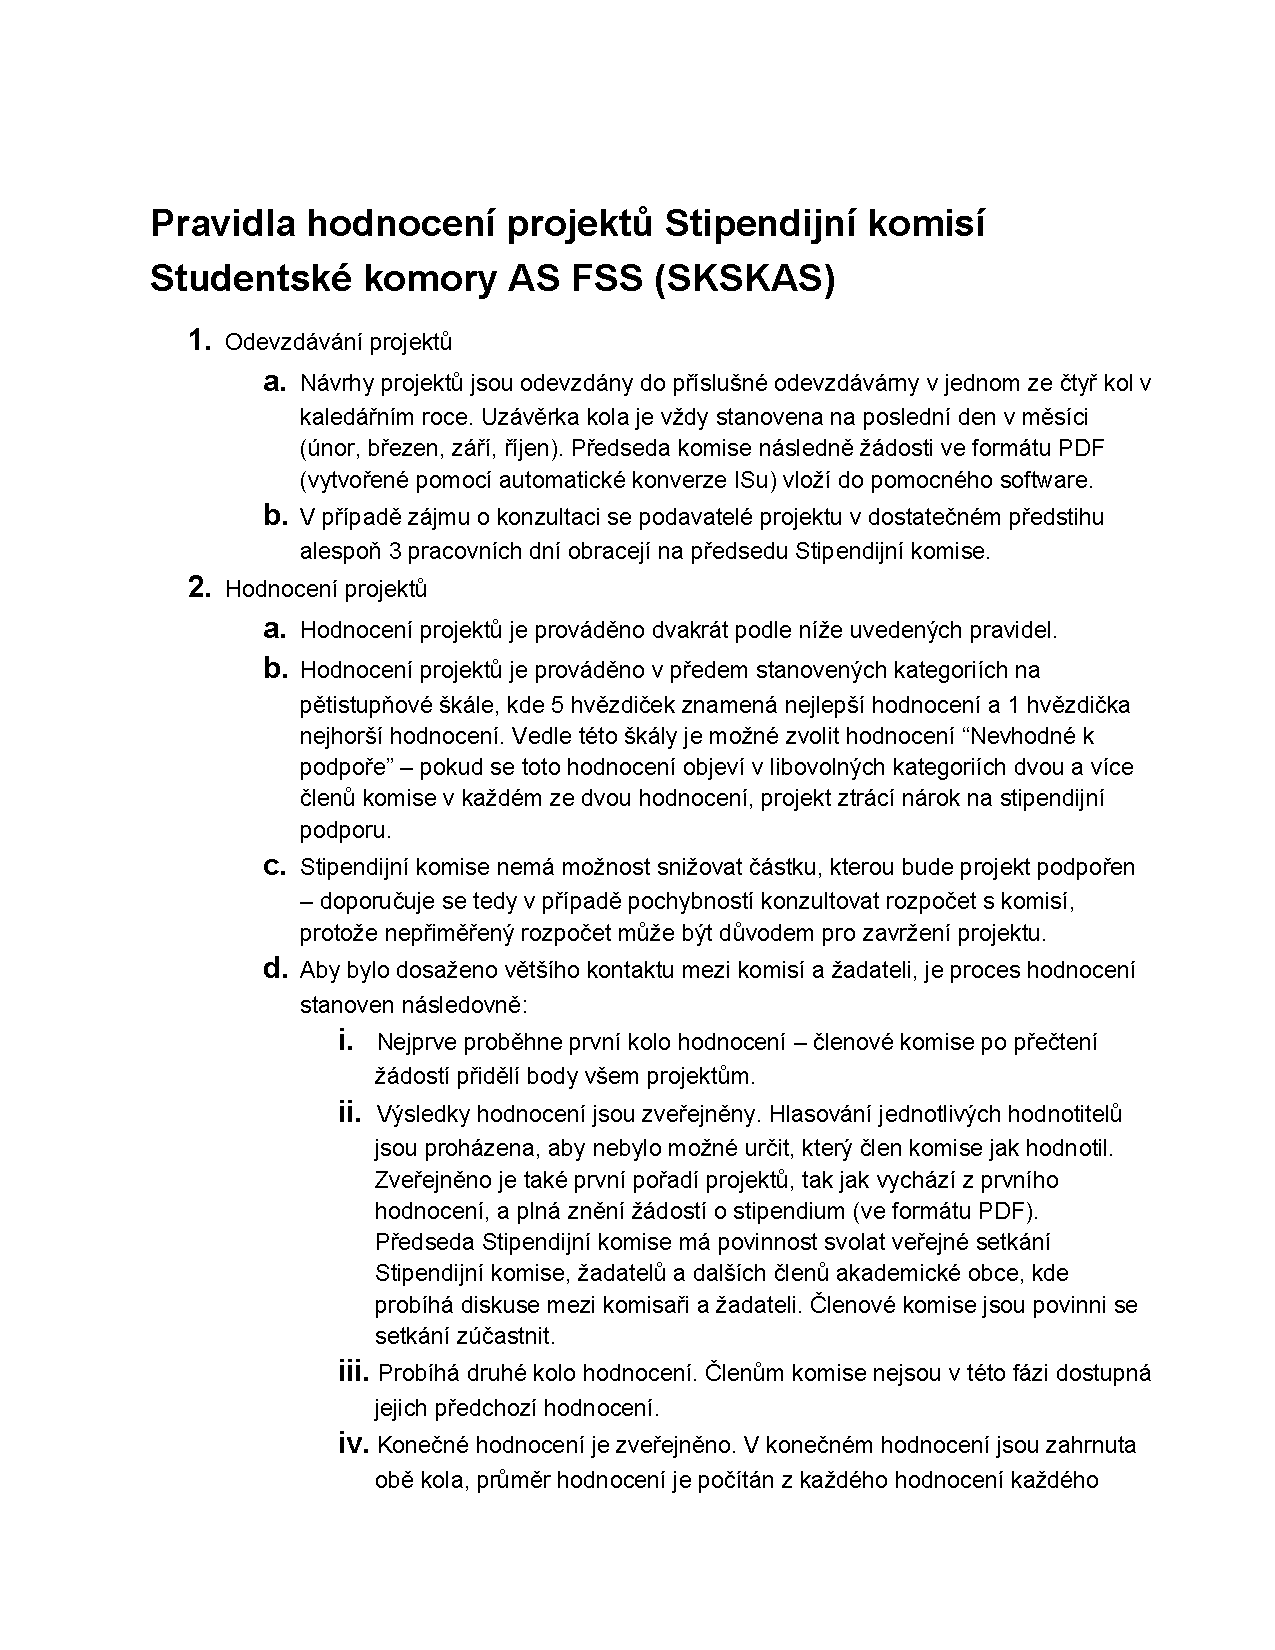
\includepdf[pages={1,2}]{pravidla-fungovani-pouze-procedura.pdf}

\cleartoleftpage
\section{Příloha B: Pravidla fungování komise sepsaná SK AS}

\includepdf[pages={1,2}]{pravidla-fungovani-prvotni-verze.pdf}

\cleartoleftpage
\section{Příloha C: Pravidla fungování komise upravená Stipendijní komisí}

\includepdf[pages={1,2,3,4}]{pravidla-fungovani-konecna-verze.pdf}

\cleartoleftpage
\section{Příloha D: Pokyny k žádosti o přiznání stipendia FSS v roce 2013}
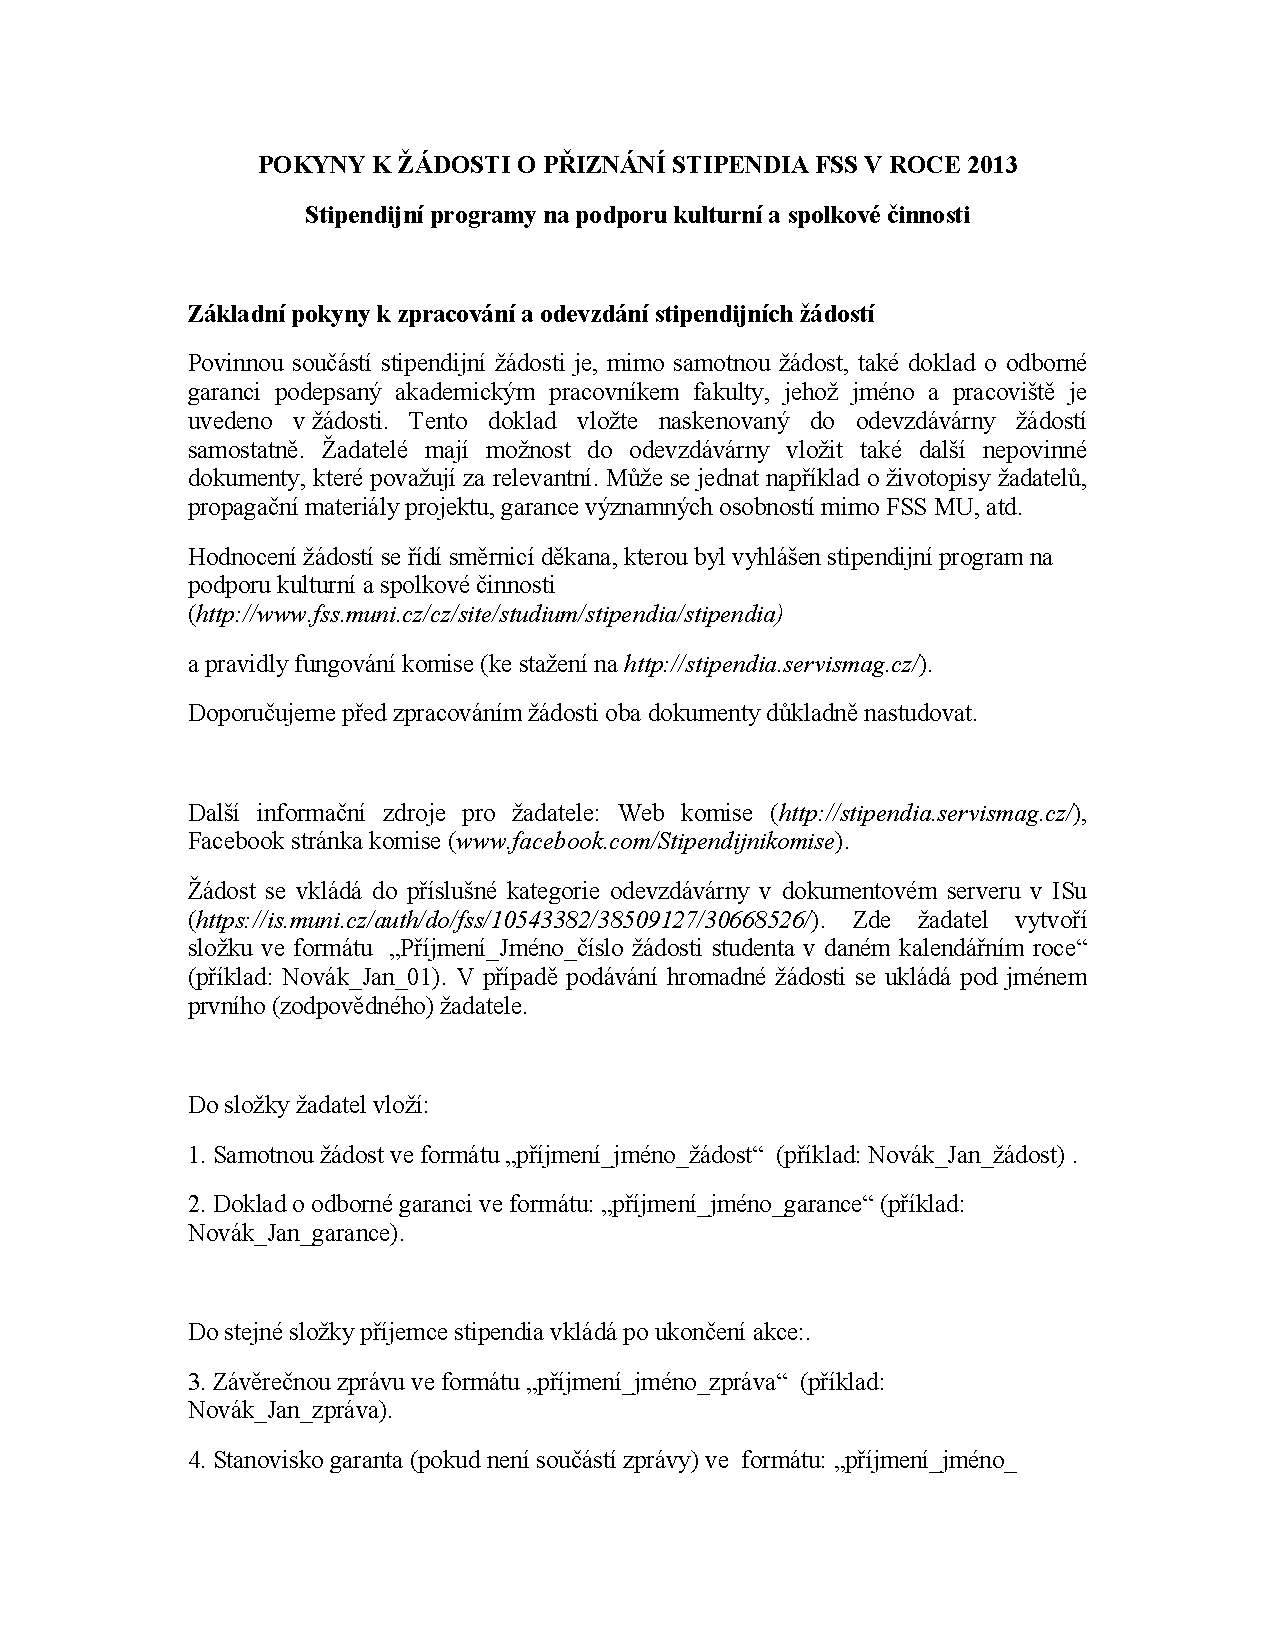
\includepdf[pages={1,2,3}]{pokyny-k-zadosti.pdf}

\cleartoleftpage
\section{Příloha E: Žádost o přiznání stipendia na FSS 2012}

\includepdf[pages={1,2}]{zadost-2012.pdf}

\cleartoleftpage
\section{Příloha F: Žádost o přiznání stipendia FSS 2013}
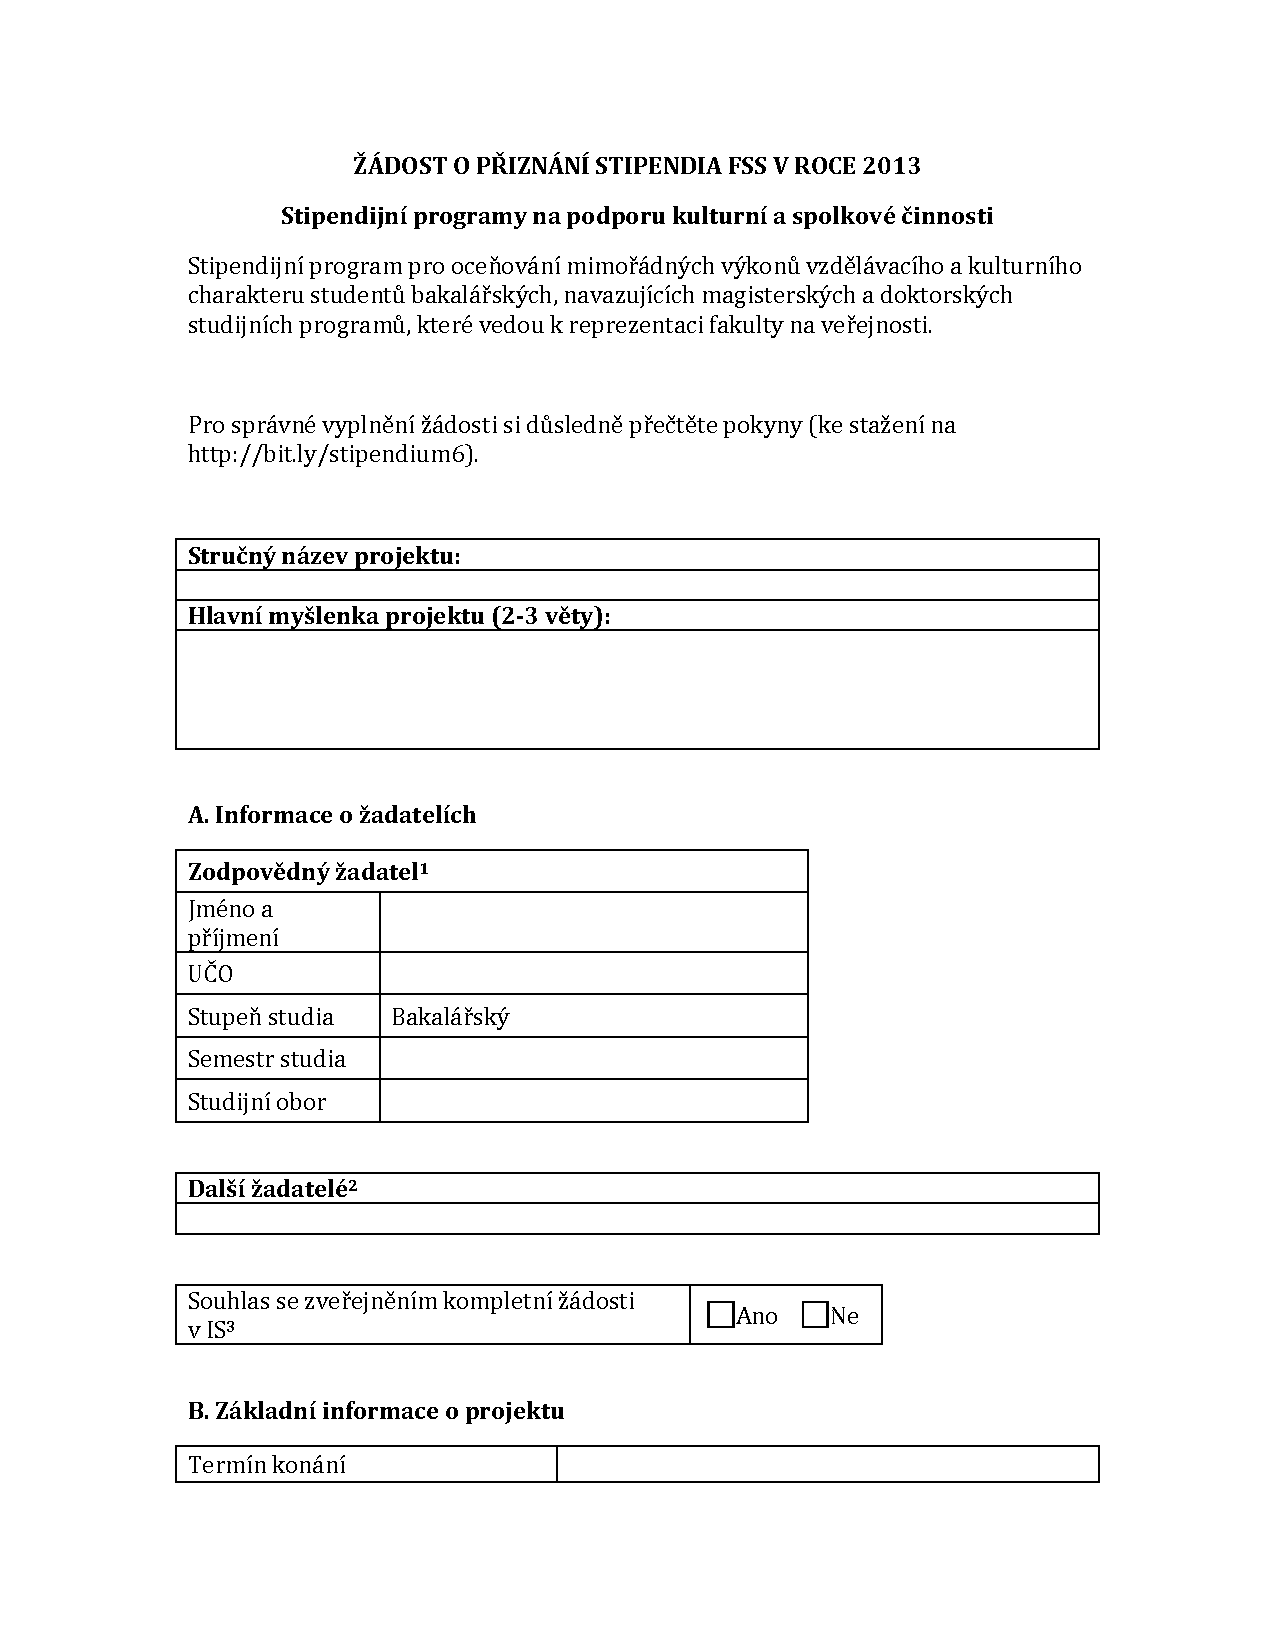
\includepdf[pages={1,2,3}]{zadost-2013.pdf}

\cleartoleftpage
\section{Příloha G: První záznam o pravidlech komise}

\includepdf[pages={1}]{prvni-zaznam-pravidel.pdf}

\cleartoleftpage
\section{Příloha H: Poznámky ze schůzky s komisí po prvním semestru}
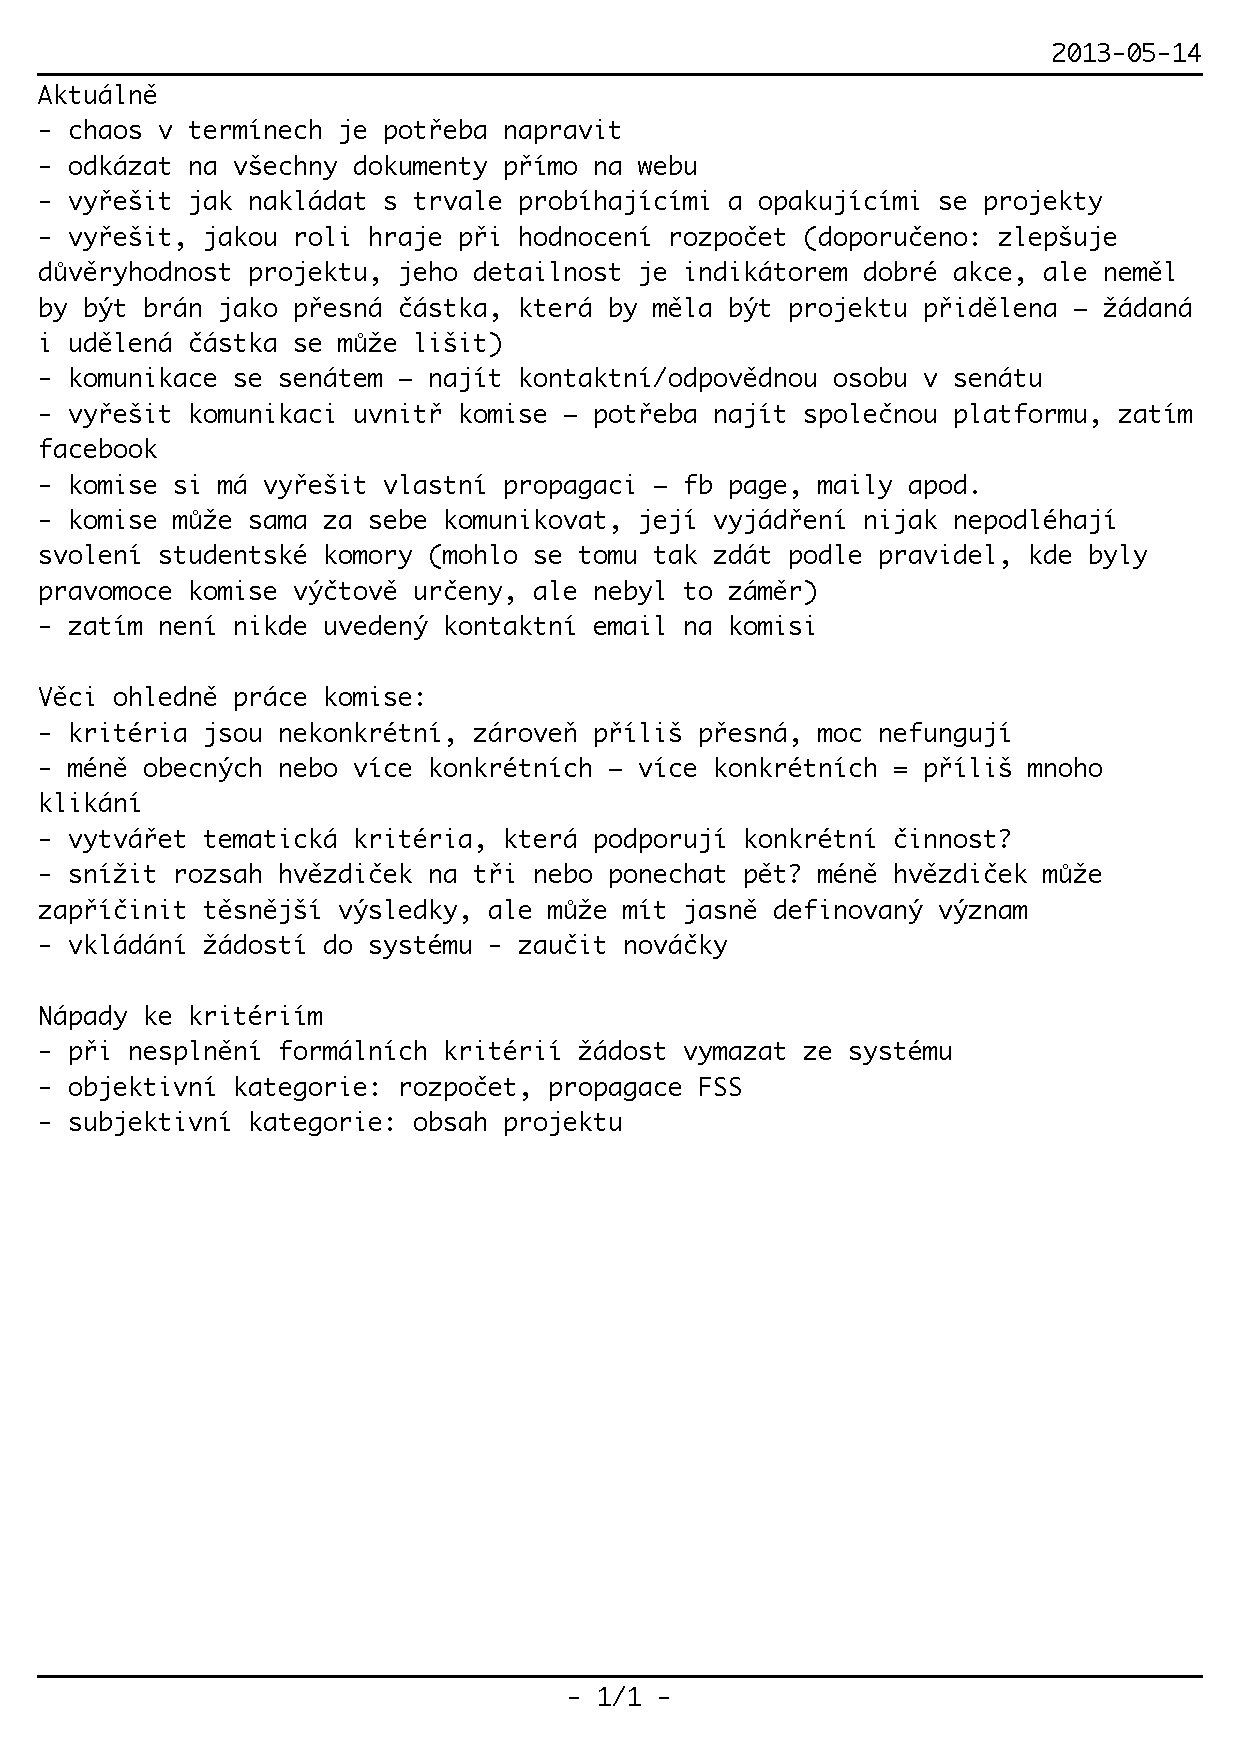
\includepdf[pages={1}]{konec-semestru.pdf}

\cleartoleftpage
\section{Příloha I: Výsledná hodnocení projektů a stav podpory}

h1 = první bodové hodnocení \newline
!1 = počet nedoporučení k podpoře v prvním hodnocení \newline
p1 = předběžný výsledek \newline
h2 = druhé bodové hodnocení \newline
!2 = počet nedoporučení k podpoře ve druhém hodnocení
t = průměr z obou hodnocení \newline
p2 = konečný výsledek (ano = podpořeno, ne = odmítnuo, chybí = nedostatečné zdroje v daném stipendijním kole)
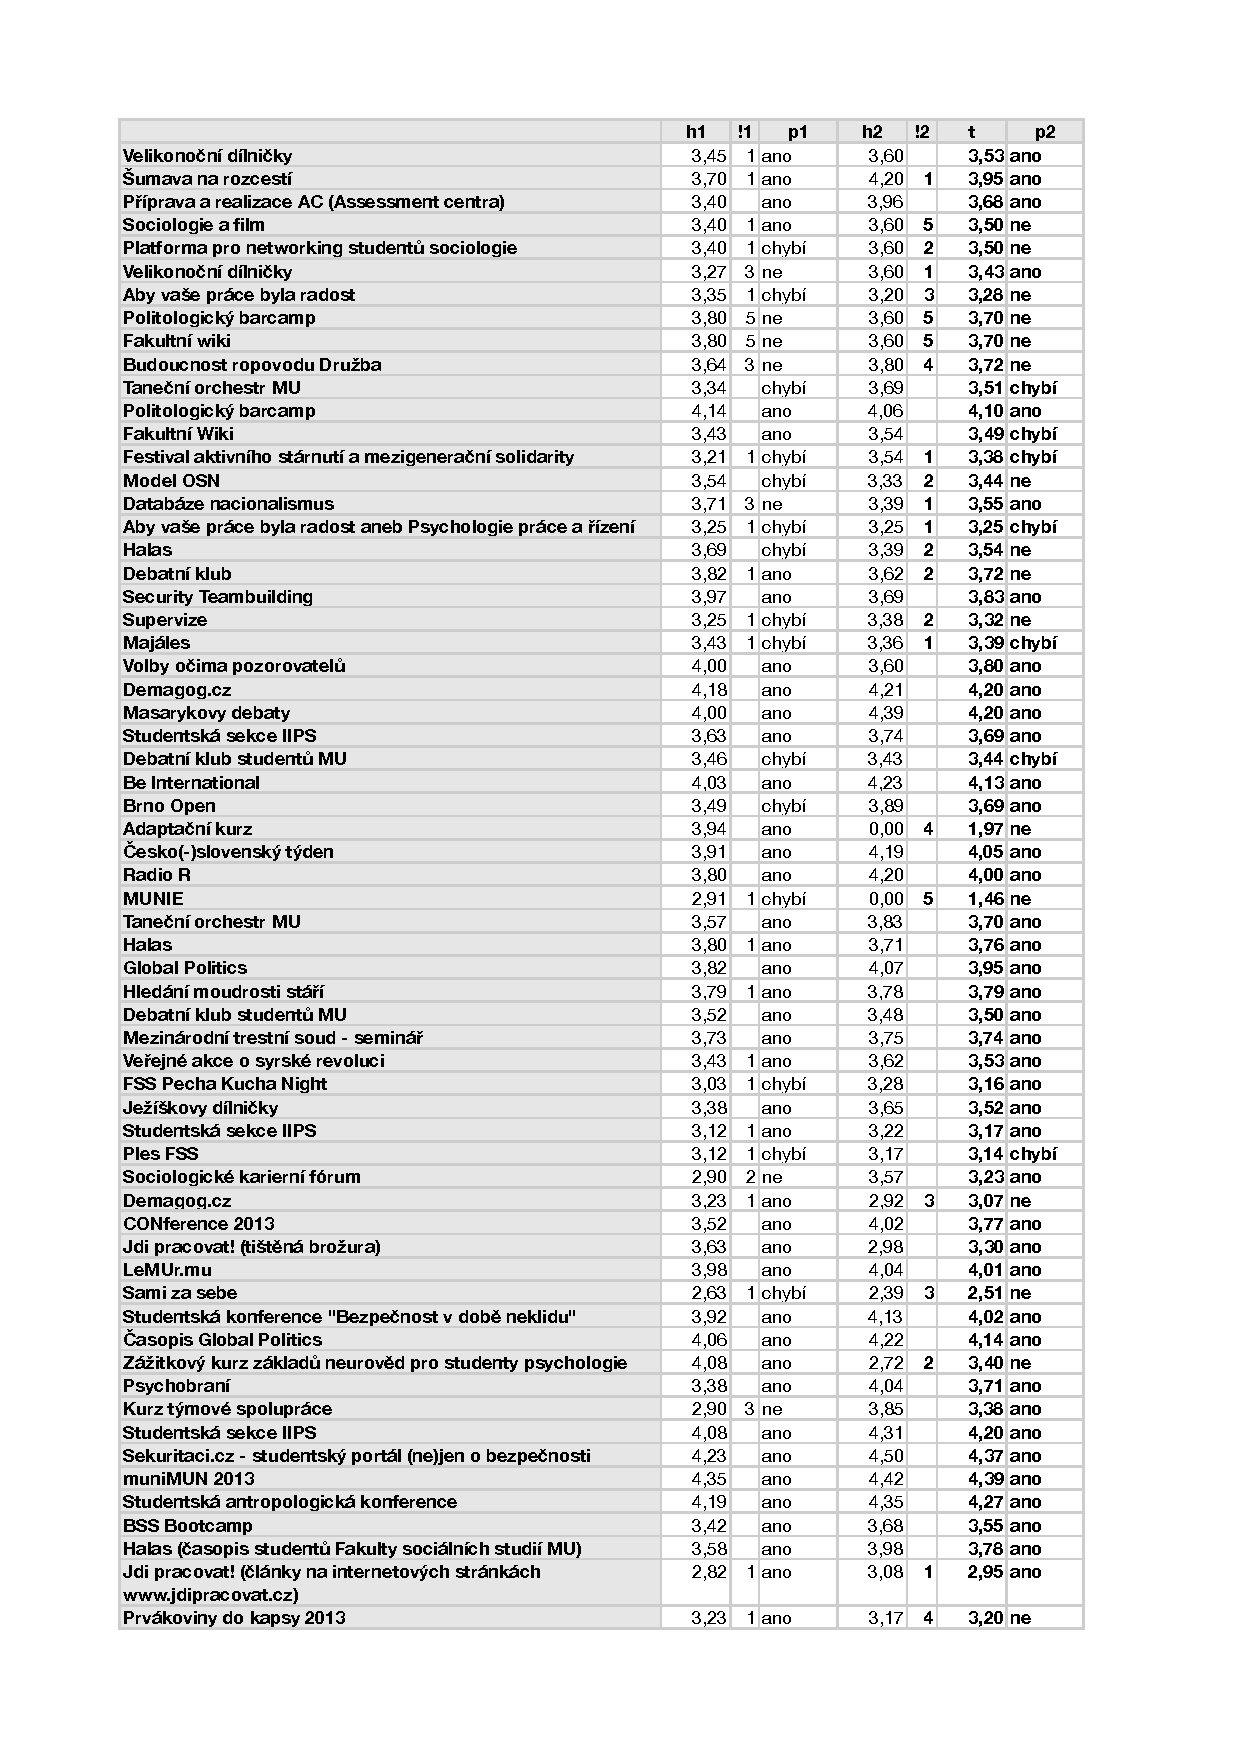
\includepdf[pages={1}]{vysledky-absolutni.pdf}

\cleartoleftpage
\section{Příloha J: Výsledná hodnocení projektů a jejich odchylky}
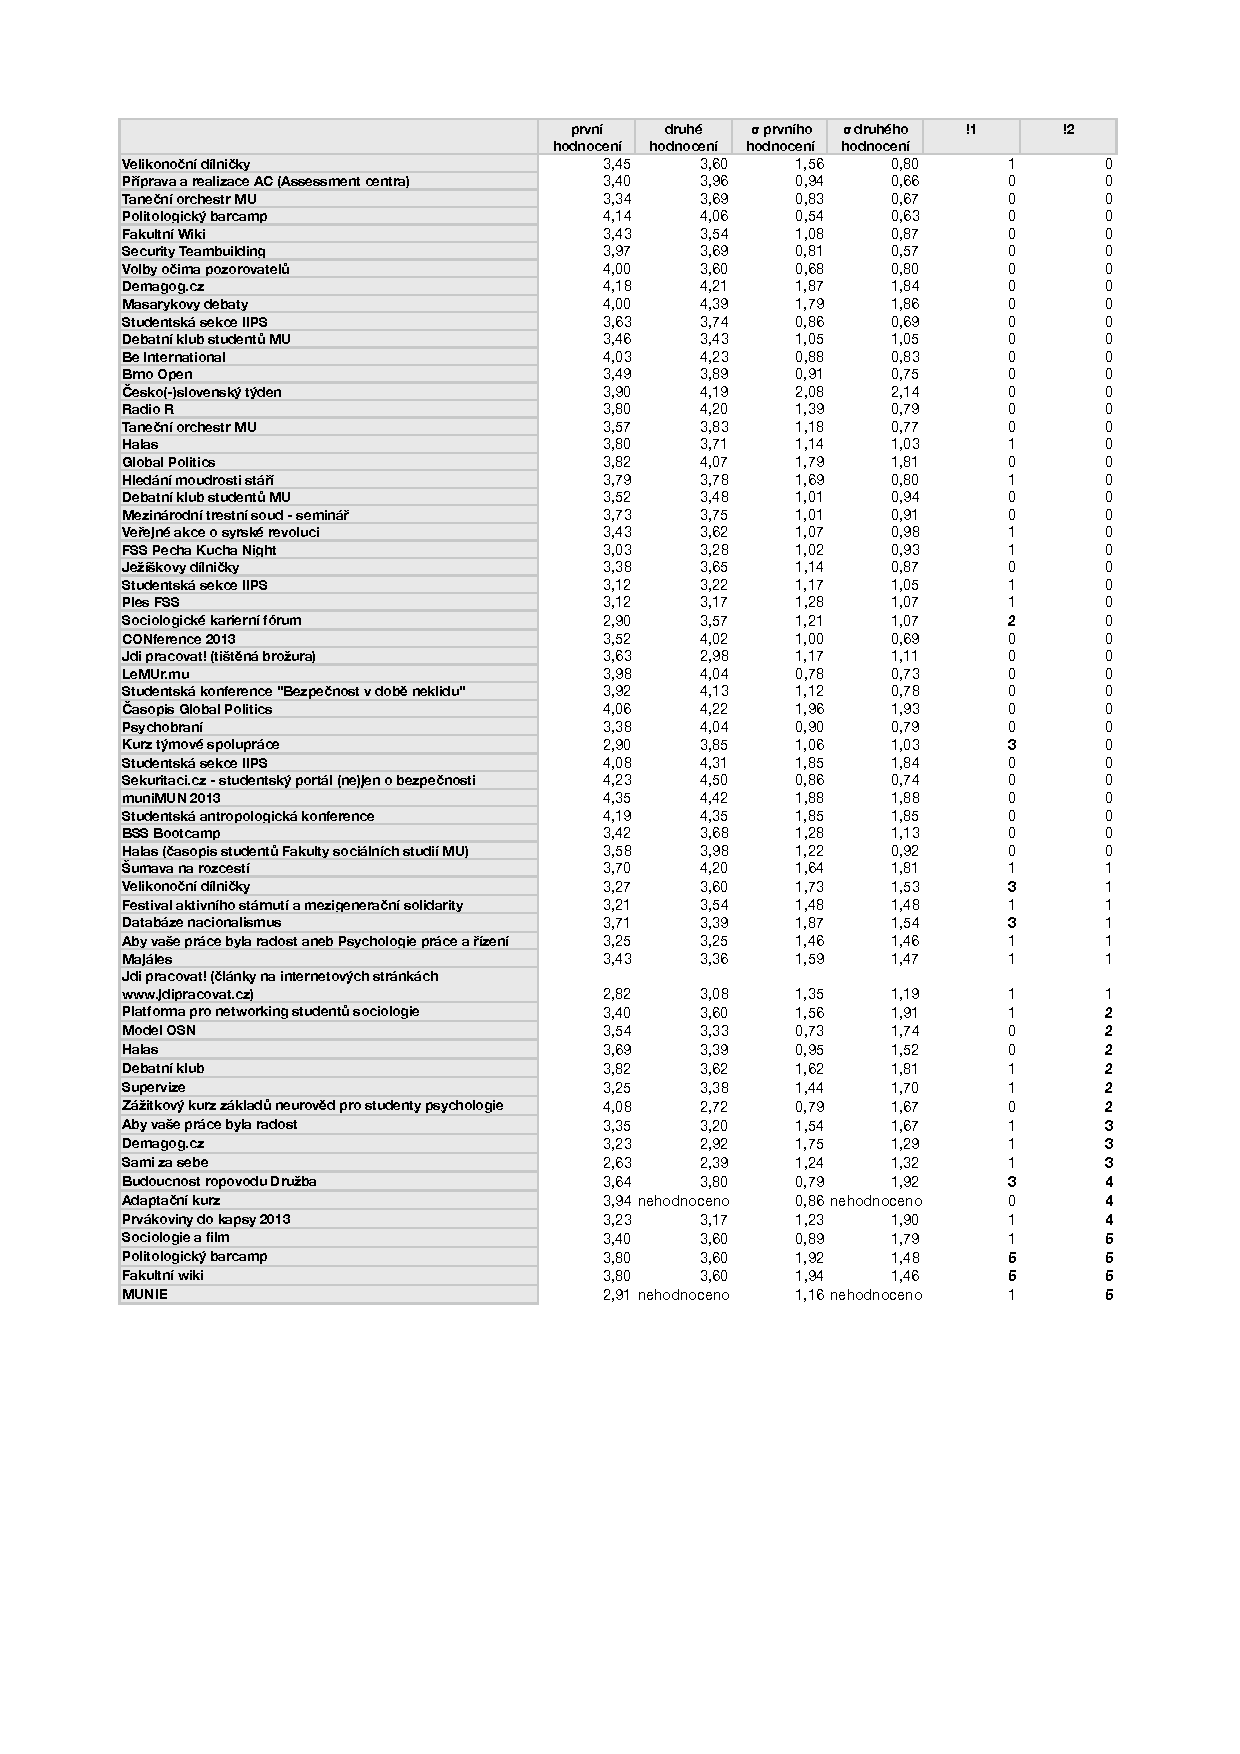
\includepdf[pages={1}]{vysledky-rozptyl.pdf}







